% !TEX root = main.tex

\chapter{Images and Video}

\section{Images}

We parse the optional argument to \texttt{includegraphics}. The \texttt{Image} class has an attribute \texttt{width} expressed as a percentage. This is computed from the (optional) \texttt{scale} or \texttt{width} parameters passed to \texttt{includegraphics}.

\begin{itemize}
\item \autoref{fig:acapb} is the original (scale = 0.25).
\item \autoref{fig:acapb-big} is the big one (scale = 0.5).
\item \autoref{fig:acapb-small} is the small one (scale = 0.1).
\item \autoref{fig:setops-subfig} shows a figure layout using \texttt{subfigure}.
\item \autoref{fig:setops-tabular} shows a figure layout using \texttt{tabular}. %The optional parameter to \texttt{includegraphics} is \texttt{scale=0.4}, and the pictures take up 40\% of each cell, which is a pity.
\end{itemize}

\begin{figure}[ht]
\centering
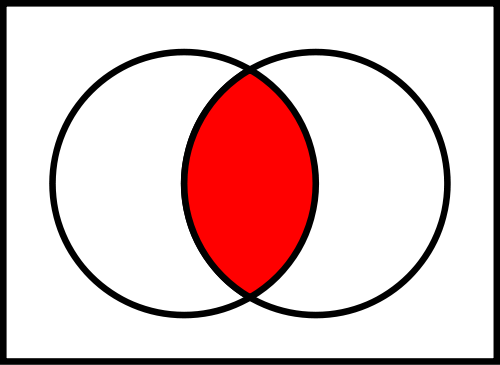
\includegraphics[scale=0.25]{AcapB}
\caption{Set intersection (scale=0.25)\label{fig:acapb}}
\end{figure}

\begin{figure}[ht]
\centering
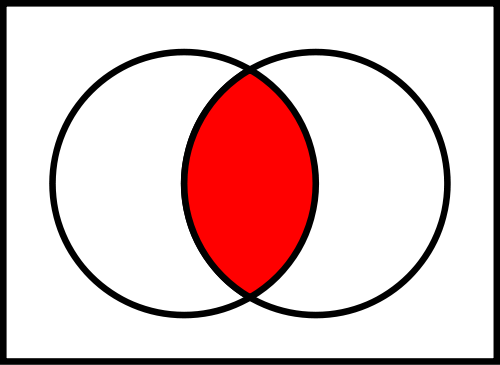
\includegraphics[scale=0.5]{AcapB}
\caption{The big one (scale=0.5)\label{fig:acapb-big}}
\end{figure}

\begin{figure}[ht]
\centering
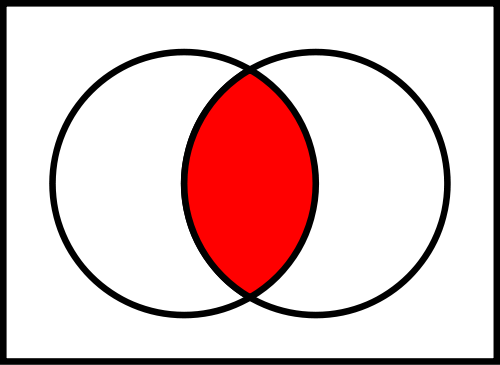
\includegraphics[scale=0.1]{AcapB}
\caption{The small one (scale=0.1)\label{fig:acapb-small}}
\end{figure}

\begin{figure}[htb]
\centering
\subfigure[Union]{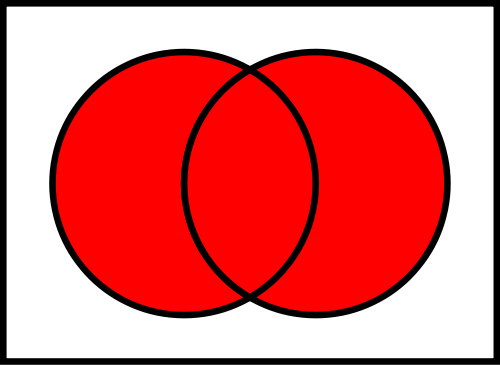
\includegraphics[scale=0.25]{AcupB}\label{fig:union}}
\subfigure[Intersection]{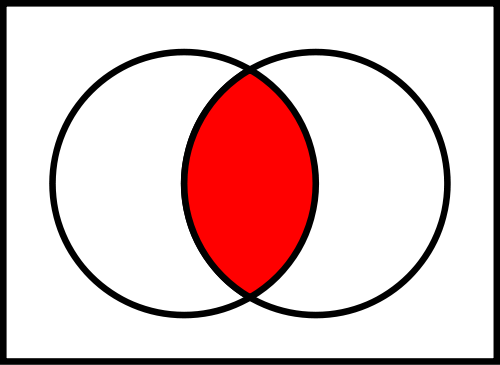
\includegraphics[scale=0.25]{AcapB}\label{fig:intersection}}
\subfigure[Complement]{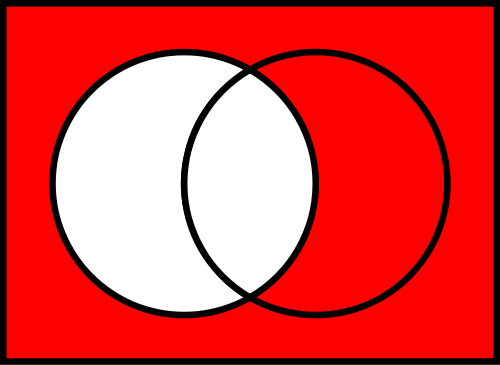
\includegraphics[scale=0.25]{Acomp}\label{fig:complement}}
\caption{Three figures using \texttt{subfigure}.\label{fig:setops-subfig}}
\end{figure}

\begin{figure}[htb]
\centering
\begin{tabular}{ccc}
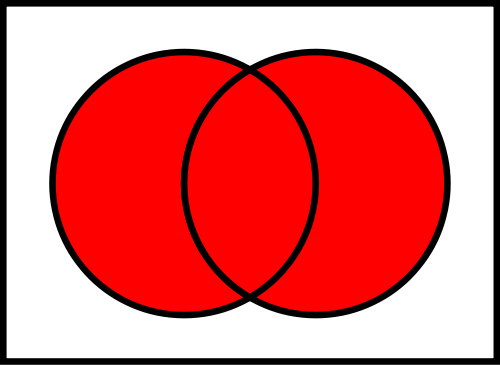
\includegraphics[width=0.25\linewidth]{AcupB} &
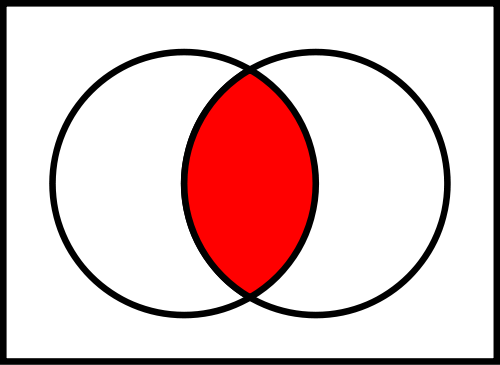
\includegraphics[width=0.25\textwidth]{AcapB} &
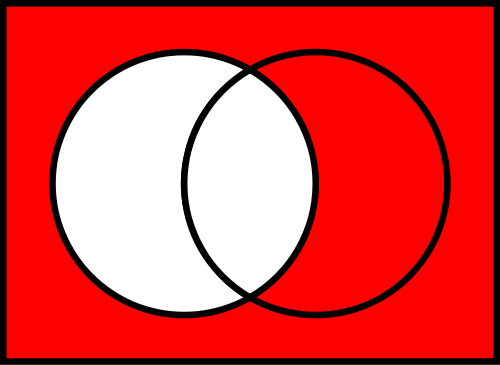
\includegraphics[width=0.25\textwidth]{Acomp} \\
(a) Union & (b) Intersection & (c) Complementation \\
\end{tabular}
\caption{Three figures using \texttt{tabular}.\label{fig:setops-tabular}}
\end{figure}

%--------------------
\section{Videos}
Embedding videos in PDFs is not easy and not recommended. Instead we include hyperlinks links using the \texttt{url} and \texttt{href} macros. 


\subsection{The \texttt{url} macro}
Please watch this video: \url{https://www.youtube.com/watch?v=oCDXhvXye9E}.

\subsection{The \texttt{href} macro}
Please watch this \href{https://www.youtube.com/watch?v=oCDXhvXye9E}{video} on YouTube.

\subsection{The \texttt{video} environment}
Here is a floating {\tt video} environment which uses the custom {\tt includevideo} command. This command is intended to mirror the way that {\tt includegraphics} is used within a floating {\tt figure} environment. In the PDF version this is again rendered as a hyperlink, but {\tt LatexTree} embeds the video into the webpage. To get an embed code for a YouTube video, click on {\tt Share} underneath the video then {\tt Embed} and it will generate an entire iframe tag. You can recover the url from this quite easily.

\begin{video}
\centering
\includevideo[scale=0.5]{https://www.youtube.com/embed/oCDXhvXye9E}
\caption{Listen and learn folks!\label{vid:och}}
\end{video}

\endinput

